\documentclass[a4paper]{article}

\usepackage{graphicx}
\usepackage{multirow}
\usepackage{cite}
\usepackage{amsmath,amssymb,amsfonts}
\usepackage{algorithmic}
\usepackage{graphicx}
\usepackage{textcomp}
\usepackage{color}
\usepackage{upgreek}
\usepackage{listings} 

\newcommand{\sbr}[1]{\left[#1\right]}
\newcommand{\br}[1]{\left(#1\right)}
\newcommand{\cbr}[1]{\left\{#1\right\}}
\newcommand{\abr}[1]{\left|#1\right|}
\newcommand{\exbr}[1]{\left\langle #1 \right\rangle}
\newcommand{\nbr}[1]{\left\lVert #1 \right\rVert}

\newcommand{\fNorm}{\mathcal{N}}
\newcommand{\MidBar}[1]{{\ooalign{\hfil$#1$\hfil\cr\kern0.08em--\hfil\cr}}}
\newcommand{\sC}{\mathbb{C}}
\newcommand{\ci}{\mathbf{i}}
\newcommand{\sN}{\mathbb{N}}
\newcommand{\sR}{\mathbb{R}}
\newcommand{\sL}{\mathit{\Lambda}}
\newcommand{\sG}{\mathit{\Gamma}}
\newcommand{\sSS}{\mathit{\Omega}}
\newcommand{\sE}{\mathcal{E}}
\newcommand{\sFW}{\mathfrak{W}}
\newcommand{\sFB}{\mathfrak{B}}
\newcommand{\sFF}{\mathfrak{F}}
\newcommand{\sFX}{\mathfrak{X}}
\newcommand{\sFP}{\mathfrak{P}}
\newcommand{\Open}[1]{\mathfrak{O}(#1)}
\newcommand{\Close}[1]{\mathfrak{A}(#1)}
\newcommand{\sComp}[1]{{#1}^{c}} 
\newcommand{\sIn}[1]{{#1}^{i}} 
\newcommand{\sAd}[1]{{#1}^{a}} 
\newcommand{\sOp}[2]{{#1}^{#2}} 
\newcommand{\rt}{\mathbf{t}}
\newcommand{\ReLU}{\mathrm{ReLU}}
\newcommand{\rx}{\mathbf{x}}
\newcommand{\trx}{\tilde{\mathbf{x}}}
\newcommand{\rf}{\mathbf{f}}
\newcommand{\rv}{\mathbf{v}}
\newcommand{\ry}{\mathbf{y}}
\newcommand{\rz}{\mathbf{z}}
\newcommand{\card}{\mathrm{card}}
\newcommand{\od}{\mathrm{d}}
\newcommand{\cpi}{\uppi}
\newcommand{\ORe}{\mathrm{Re}}
\newcommand{\OIm}{\mathrm{Im}}

\newcommand{\hpsi}{{\hat{\psi}}}
\newcommand{\hphi}{{\hat{\phi}}}
\newcommand{\hatp}{{\hat{p}}}
\newcommand{\hatq}{{\hat{q}}}
\newcommand{\hatj}{{\hat{j}}}
\newcommand{\jbar}{{\MidBar{j}}}
\newcommand{\hatM}{{\hat{M}}}
\title{Mathematical description and parallelization of QAOA system}
\date{March, 2026, 31st}
\begin{document}
\maketitle
In this document we describe components of QAOA system mathematically, and introduce a novel parallelization algorithm for QAOA system. I, Shibata, supposes futher discussion to improve and expand the QAOA system needs basic symbols and formulas to define it. Therefore, I wrote an article here. Pleaes tell me any suggestion easily.

\section{Address for 1st qubit mixer operation}
Indexes are critical to implement the QAOA system precisely on FPGAs, rathar than matrix-vector expression because we must calculate equivalent index expressions when those matrix operation is implemented on ogical circuit. So, the indexing and its relation to operation is defined strictly, from actual easy example to general case.

Let \(N\) be a number of qubits, \(D=2^{N}\) be a dimension of state vector. Let \(\psi\in\sC^D\) be a state vector, and let \(p\) be a index of element of \(\psi\). Then \(p\) take a form of,
\begin{equation}
    \label{e1}
p = p_N \cdots p_2p_1 = \sum_{i=1}^N p_i 2^{i-1},
\end{equation}
where \(p_i\in \{0, 1\}\) is an each bit of \(p\). So we can see the number of all possible value of such \(p\) is \(2^N\), that equals to \(D\). 

We expree any integer between \(0, D-1\) in the format \eqref{e1} seemlessly. That is, if we write
\[
    p = 0000\cdots00101,
\]
then, we also write its identical express using decimal integer \eqref{e1}, 
\[
    p = 5.
\]
Considering the series of integer sequence \(j=0,1,...,D/2-1\), and a state vectors \(\psi\), we can determine 2 indexes for mixier operation in the case of 1st qubit as,
\begin{equation}
    \label{ei}
    p = 2 j, q = 2 j + 1.
\end{equation}
Letting \(p, q\) have the following binary expression,
\[
 p = p_N \cdots p_2 p_1, q = q_N \cdots q_2 q_1,
\]
then we can see for all \(i = 1,2,...,N\),
\[
\begin{matrix}
    i = 1\Rightarrow p_i \neq q_i\\
    i\neq 1\Rightarrow p_i = q_i
\end{matrix}
\]
So the mixer operation will be,
\begin{align}
    \nonumber
    \psi_p &= \psi_p\cos\beta - \ci\psi_q \sin \beta \\
    \label{em}
    \psi_q &= -\ci\psi_p\sin \beta  + \psi_q\cos \beta
\end{align}
\section{Addressing for general case of mixer operation}
To get 2 index for general case of mixer operation, there are several way of addressing. In this section, we introducing a method with swaping 2 bit in a index variable used in the case of 1st qubit mixer operation described in the previous section.

Let \(n\) be a current qubit place we are focusing on for mixer operation, \(\hat{p}, \hat{q}\) be indexes of state vector element that should be applied a mixer operation. Assuming we have index expression,
\begin{equation}
    \label{e4}
    p = p_N\cdots p_n\cdots p_2p_1, q = q_N\cdots q_n \cdots q_2q_1
\end{equation}
we obtain \(\hat{p}, \hat{q}\) as,
\begin{equation}
    \hat{p} = p_N \cdots p_1\cdots p_2 p_n, \hat{q} = q_N \cdots q_1\cdots q_2 q_n.
\end{equation}
Now, we see easily,

then we can see for all \(i = 1,2,...,N\),
\[
\begin{matrix}
    i = 1\Rightarrow \hatp_i \neq \hatq_i\\
    i\neq 1\Rightarrow \hatp_i = \hatq_i
\end{matrix}
\]
therefore, using these indexes \(\hat{p}, \hat{q}\), we do mixer operation for \(n\)-th qubit as, 
\begin{align}
    \nonumber
    \psi_\hatp &= \psi_\hatp\cos\beta - \ci\psi_\hatq \sin \beta,\\
    \label{emg}
    \psi_\hatq &= -\ci\psi_\hatp \sin \beta  + \psi_\hatq \cos \beta,
\end{align}
where \(\ci^2 = -1\).
\subsection{Invariance on exchange of qbits for mixer operation}
\label{mixerInvariance}
We further formalize mixer operation here. The sets of index pairs that the mixer operation applied is denoted as \(S_1, ...,S_N\) such that,
\[
    S_n = \cbr{(p, q)| P(p, q, n)}, P(p, q, n) \Leftrightarrow p_i\neq q_n \forall i\neq n \br{p_i = q_i}
\]
If we have a serise \(p^{kn}, q^{kn}, k=1,2,...,2^{N-1}, (p^{kn}, q^{kn})\in S_n\) where each pair is distinct each other, then, the processing of mixer operation can be,
\begin{align}
    \psi_{p^{kn}}' &= \psi_{p^{kn}}\cos\beta - \ci\psi_{q^{kn}} \sin \beta, \\
    \label{emg2}
    \psi_{q^{kn}}' &= -\ci\psi_{p^{kn}} \sin \beta + \psi_{q^{kn}} \cos \beta.
\end{align}
we can exchange any \(n\) and \(m\) in the series. 

Proof: In the case we apply \(n,m, n\neq m\)-th qbit is considered. If we apply in the order of \(m, n\), for any \(p=0,1,...,D/2-1\), there uniquly exists pairs \((p, q)\in S_{m}, (p, a), (q, b)\in S_{n}\) from the definition of \(S_n\). And because  operator of \(n\)-th qbit is already applied, then,

\begin{align}
    \nonumber
    \psi_{p}' &= \psi_p \cos\beta - \ci\psi_q \sin \beta, \\
\end{align}
But because operation for \((p, a), (q, b)\) have been done already, we can substitute its result, therefore, obtain
\begin{align}
    \nonumber
    \psi_{p}' &=  (\psi_{p}\cos\beta - \ci\psi_{a} \sin \beta)\cos\beta - \ci(\psi_q \cos \beta - \ci \psi_b \sin \beta) \sin \beta, \\
    \label{eqn2m}
    & = \psi_p\cos^2 - \psi_b\sin^2\beta - \ci\br{\psi_a \sin\beta\cos\beta + \psi_q\cos\beta\sin\beta}.
\end{align}
where \(p\neq q, a\neq b\). 

Before going to the opposite case, we see \((a, b)\in S_{m}\).

Proof: we have,
\begin{align*}
    &a_n \neq p_n\land \forall i\neq n(a_i = p_i), \quad\because (p, a)\in S_n,\\
    & b_n \neq q_n\land \forall i\neq n(b_i = q_i), \quad\because (q, b)\in S_n, \\\
    &q_m\neq p_m\land\forall i\neq m (q_i=p_i), \quad\because (p, q)\in S_m.
\end{align*}
The above logic provides, \(a_m = p_m, b_m = q_m, q_m\neq p_m\)  and \(n\neq m\), that is, from the transitive law \footnote{\(x = y, y=z\Rightarrow x=z\)} of equation, \(a_m \neq b_m\). In addition, for all \(i\neq m\), if \(i\neq n\) then \(a_i = b_i\). For \(i\neq m \land i=n\), if we assume \(a_n\neq b_n\), because these takes only 2 kind of values 0 or 1, it can be expressed as \(a_n = Q, b_n = Q*, Q** = Q.\). Now \(a_n\neq p_n, b_n\neq q_n\), so \(p_n = Q*, q_n = Q\). But \(p_n= q_n\) should holds for the third logic of qubit. To solve this contradiction, we must say \(a_n = b_n\). Therefore in sammary, 
\[
 a_m \neq b_m\land \forall i\neq m\br{a_i=b_i}.
\]
It means \((a, b)\in S_m\).

Then in the opossite case, for the same indexes \(p, q, a, b\),
\begin{align}
    \psi_{p}' &= \psi_p\cos\beta - \ci \psi_a \sin \beta
\end{align}
Here, we know \((p, q), (a, b)\in S_m\), therefore,
\begin{align}
    \nonumber
    \psi_{p}' &= (\psi_p\cos\beta - \ci \psi_q \sin \beta)\cos\beta - \ci (\psi_a\cos\beta - \ci \psi_b \sin \beta) \sin \beta, \\
    \label{eqm2n}
    &= \psi_p \cos^2\beta - \psi_b\sin^2\beta -\ci\br{\psi_q\sin\beta\cos\beta + \psi_a\cos\beta\sin\beta}.
\end{align}

Because applying mixer operation in order of \(n, m\) (\eqref{eqn2m}) and that in order of \(m, n\) (\eqref{eqm2n}) give the same result, any pair of mixer operation to adjacent qbits are commute. Because it is well known any permutation can be expressed with the finite combinations of such adjacent exchange, from the mathematical induction, any sequence of qbit order to apply mixer operation gives the identical result. 

\section{Pipeline element}
\label{spipe}
This section formalize a timing of the pipeline as a mathematical functions. The reason both cost function and mixer operator can be computed using the same pipeline introduced here is also explained end of the section.

Let \(T\) be a number of pipeline stages, then for \(j=1,2,...,D-1\), the pipeline is defined using the variables \(\phi, c, s, \xi, A\). Meanings are,
\begin{itemize}
    \item \(\phi\): amplitude of the state vector
    \item \(c\): Value of cosine or real part of cost function operator
    \item \(s\): Value of sine or imaginary part of cost function operator
    \item \(\xi\): Switch flag of first componet of amplitude or that of second, or cost function.
    \item \(A\): Index (Address) of the amplitude place to be stored.
\end{itemize}
These variables form a serise, like in a way, \(\phi_1, \phi_2, ..., \phi_T\), where  \(T\) is the number of pipeline depth. Subscript of \(1\) like \(\phi_1\) means input stage. This document use \('\) to indicate the next state in terms of discrete time on the clocks, like in a way \(\phi'\). 

Here, for example, to compute the mixer operation, the input is set as,
\begin{equation}
    \label{eminit}
    \begin{matrix}
        \phi_{1}' = \psi_\hatj\\
        c_1' = \cos\beta\\
        s_1' = \sin\beta\\
        \xi_1' = 0j_0\\
        A_1 = \hatj
    \end{matrix} 
\end{equation}

The meaning of precedent \(0\) for \(\xi\) is explained in the reuse method of this unit for cost function operation later. First this document describes the use in mixer operation.
Updating the pipeline values as,
\[
    \br{\phi, \xi, A, c, s}'_{\tau +1} = \br{\phi, \xi, A,c,s}_{\tau}, \tau=1,2,...,T
\]  
then complex number operation is defined as following.
\begin{align}
    \label{ep00}
    \psi_{A_{T}}' &= \xi_{T} - \zeta_{T-1} &\Leftarrow \xi_T = 00\\
    \label{ep01}
    \psi_{A_{T}}' &= -\zeta_{T+1} + \xi_{T} &\Leftarrow \xi_T = 01\\
    \label{ep10}
    \psi_{A_{T}}' &= \xi_{T} +  \zeta_{T} &\Leftarrow \xi_T = 10
\end{align}
where, 
\begin{equation}
    \xi_{\tau} = \phi_\tau c_\tau, \zeta_\tau = \ci\phi_\tau  s_\tau
\end{equation}
must be calculated with 4 multipliers (note that there are 2 real and complex value multiplications).
The notation \('\) means updated value, i.e., if we denote the time stamp as \(t\in\sN\), then \(\psi' = a\) means \(\psi^{t+1} = a^t\) in this context.

This pipline can be used also for cost function operation. For this, we set the inital values in the pipeline system as,
\begin{equation}
    \label{ecinit}
    \begin{matrix}
        \phi_{1}' = \psi_j\\
        c_1' = \ORe(H_j)\\
        s_1' = \OIm(H_j)\\
        \xi_1' = 10\\
        A_1 = j
    \end{matrix} 
\end{equation}
When we apply the input with \eqref{eminit}, \eqref{ep00} and \eqref{ep01} is applied alternately to get a result for 2 mixed amplitude in this order. That is, setting \eqref{eminit} make the pipeline calculate 2 mixer operation with 2 clocks. The throughput is 1 per 1 clock. On the other hand, when we apply the input with \eqref{ecinit}, only \eqref{ep10} is applied 

\section{Addressing for parallel processing}
Letting \(K=2^M\) be a number of parallell blocks. In naive inplementation, if we paralellized the system in \(K=2^M\) blocks, the system need inter local memory (like BRAMs) access \(M\)-times both for read and write. The implementation describes here reduce it to \(1\) regardless \(M\). Whole blocks works parallelly and there is no serial processing in this implementation iether. Fundamental idea to this tricky implementation is that, it re-arrage memory assignment for each amplitude of the state vector at the time of transfor for graear qbits that is used to divide the system into blocks (such qbits refers to global qbits here.), At the time of transfer.

We prepare \(K\) pipeline defined in the section \ref{spipe}. Serise of index used in each blocks are all the same.
\[
    j=0,1,...,\frac{D}{2K}-1. 
\]
For \(n=0,1,...,N-1\), we obtain \(\hatj\) here as well. The address in the view of global memory then bocome,
\[
    \jbar = kj
\]
For intuition, consider the case \(k = 5=101, j=11001\). In this case \(\jbar = 10111001\). 

The system will re-arrange the state vector. The re-arraged state vector is noted as \(\hphi\) here. The relation between original arrangement \(\phi\) to \(\hphi\) is defined using permutation \(\sigma:\cbr{0,1}^N\to\cbr{0,1}^N\),
\begin{equation}
    \hphi_\jbar = \phi_{\sigma(\jbar)}.
\end{equation}
\(\sigma\) is defined so that it shuffle index. There are several possiblity that yeild same effect to implement \(K\) block parallelization, but for generally, for any \(\hatM \geq M\), 
\begin{equation}
    \sigma\br{p_N\cdots p_{\hatM+1} p_{\hatM}\cdots p_1} = p_{\hatM}\cdots p_1 p_N\cdots p_{\hatM+1}
\end{equation}

In these definition, we can formalize the mixer operation that provide the possible implementation for \(K = 2^M \leq 2^\hatM\) paralellization with \(K\) blocks. 

\subsection{Block Mixing Algorithm} 
\label{sBMA}
We describe an alogorithm tentatively called block mixing algorithm here after in the section. It consists of local stage and global stage.

\textit{Local stage}: letting \(j=0,1,...,2^{\hatM}-1\) be an local index, and \(k=0,1,...,2^{N-\hatM}-1\) be an global index. In the local stage, using the index,
\[
\jbar = kj
\]
mixer operation is applied. In this stage, each block of pipeline includes several \(k\), for special case of \(\hatM = M\), \(k\) is equivalent to the identification of each pipeline block.

Assuming we got \(\psi\in \sC^D\) as an initial value and got \(\hpsi\in\sC^D\) by applying mixer operation to the local qbits (qbit such that its number \(n\) satisfies \(n\leq \hatM\).). Then, let \(\hpsi'\) be a state vector that shuffled its amplitude position as,
\begin{equation}
    \label{eshuffle}
    \hpsi'_\jbar = \hpsi_{\sigma(\jbar)} , \Leftrightarrow\hpsi'_{p_N\cdots p_1}= \hpsi_{p_\hatM\cdots p_1 p_N\cdots p_{\hatM+1}}
\end{equation}
where we took the representation of,
\[
\jbar = p_N\cdots p_1.
\]
\textit{Global stage}: 
Then we apply mixer operation on the qbits of \(n =1,2,...,N-M\) to \(\hpsi'\) and we obtain \(\psi^@\). Let \(\psi'\in\sC^D\) be a final result of original order, it can be obtained,
\begin{equation}
    \label{ereverseshuffle}
\psi'_\jbar = \psi^@_{\sigma^{-1}(\jbar)}, \Leftrightarrow \psi'_{p_N\cdots p_1}= \psi^@_{p_{N-M}\cdots p_1 p_N\cdots p_{N-M+1}}
\end{equation}

Let \(\bar{\psi}\) be a result of mixer operation without global qbits. Then, we claim that,
\begin{equation}
    \label{eblockmixA}
\bar{\psi} = \psi'.
\end{equation}

\subsubsection{Sammary of Block Mixing Algorithm}
Cost of copy data exists in \eqref{eshuffle} and \eqref{ereverseshuffle}. But this copy process can be in parallell. About the amount of data to be copied, for example, \(1/K\) is remained in the original block, and elemenents amount of \(1-1/K\) should be moved to another block. But this copy is only once for shuffling (\eqref{eshuffle}) and restoring (\eqref{ereverseshuffle}), it should be the least cost among any parallel algorithm on distributed systems in this order of parallelization \(K\). If it compares to the naive implementation (Fig. \ref{f1} bottom right) in which each mixer oepration for each qbit needs access to inter BRAM, because such qbit by qbit operation needs \(M\ (K=2^M)\) times access totally, this proposed algorithm reduced the chance of global access at the ratio \(1/K\). 

Cost function operation can be applied at the stage of restoration between the period after fetching a data from another BRAM and storing it to the original position of the original BRAM. e.g., \(N=2^{20}\) which is a practical number of qbits, we can take \(\hatM=2^{10}\) which ordinally above the avaiable blocks for parallelizations. Note that taiking \(\hatM > M\), where \(M\) is number of physical blocks, is not a problem. We can see that there is no problem in such configuration \(\hatM > M\) in the mathematical proof of the algorithm later.
 
If we can set \(\hat{M} = N/2\), way of pipline do is totally the same as for both of operations on global and local qbits.
\begin{figure}
    \label{f1}
    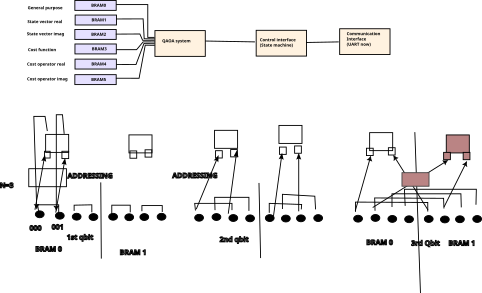
\includegraphics[width=\linewidth]{diagram.pdf}
    \caption{(Top) Block diagram of current system with only 1 pipeline. Pipeline is exists in the block of QAOA system (invisible in this figure). (Bottom) pipeline's working image to each amplitude. The pipeline takes 2 input sequentially, and it compute them using 2 clocks. So the thoughput is 1 element per 1 clock. (Bottom right) Cross part is described in the case using 2 blocks for 2 paralellization. Generalization of this example to \(K > 2\) parallelization is the main topic of this article.}
\end{figure}

\subsubsection{Proof of Block Mixing Algorithm yeilds the same result that do not use global qbits}
To prove this, we need to define mixer operation for qbit \(n\) more generally. Mixer operation on \(n\)-th qbit is expressed as \(U_n\). And from the result of invariance on mixer operation in section \ref{mixerInvariance}, we have,
\begin{equation}
    \label{emixcomm}
 U_n U_{m}\psi = U_m U_n\psi  
\end{equation}
We denote operation exchanging adjacent qbits as \(\Theta_{n, 1}\), then
we want to show,
\begin{equation}
    \label{einvn1}
    U_n \psi = \Theta_{n, 1} U_{1} \Theta_{n, 1}\psi .
\end{equation}

Proof:  \( U_n \psi\) is described as for all index \(p = 0,1,...,{D-1}, q, (p, q)\in S_n\) (such \(q\) exists uniquely),
\begin{align*}
    \br{U_n \psi}_p &= \psi_p \cos\beta - \ci\psi_q \sin \beta.
\end{align*}
When applying \(\Theta_{n,1}\), there exist indexes \(a, b=0,1,...,D-1\) that satisfy for arbitrary \(h\in\sC^D\), 
\begin{align*}
    \br{\Theta_{n, 1}h}_{p} &= h_{a}, p_N\cdots p_1 = a_N\cdots a_{n+1}a_1 a_{n-1}\cdots a_2 a_n,\\
    \br{\Theta_{n, 1}h}_{q} &= h_{b}, p_N\cdots q_1 = q_N\cdots b_{n+1}b_1 b_{n-1}\cdots b_2 b_n.
\end{align*}
Now we know \(p_n\neq q_n\) from definition, so \(a_1 \neq b_1\) holds. Similary, \(\forall i\neq n,  a_i=b_i\). It means \((a, b)\in S_1\). Therefore,
\begin{align*}
    \br{U_1 h}_{a} & = h_a \cos\beta - \ci h_b \sin \beta\quad \because (a, b)\in S_1\\
    &= \br{\Theta_{n, 1} h}_p\cos\beta - \ci\br{\Theta_{n, 1}h}_q \sin \beta.\\
   \therefore \br{\Theta_{n,1} U_1 h}_{p} & = \br{\Theta_{n, 1} h}_p\cos\beta - \ci\br{\Theta_{n, 1}h}_q \sin \beta.
\end{align*}
If we substitute \(h = \Theta_{n,1}\psi\) and applying \( \Theta_{n,1}\Theta_{n,1}\psi = \psi\), then, 
\begin{equation}
   \br{\Theta_{n,1} U_1 \Theta_{n,1}\psi }_{p}  = \br{\psi}_p\cos\beta - \ci\br{\psi}_q \sin \beta = \br{U_n \psi}_p.
\end{equation}
Therefore, \eqref{einvn1} holds.

Using \eqref{einvn1}, and letting \(U_{n, m}\) is an operator exchanging \(n\) and \(m\)-th qbit index, \(U_{n, m} = U_{n, 1}U_{m, 1}\). So we have,
\begin{equation}
    U_n \psi = \Theta_{n, 1} U_{1} \Theta_{n, 1}\psi = \Theta_{n, 1} \Theta_{m, 1} U_{m} \Theta_{1, m}\Theta_{n, 1}\psi = \Theta_{n, m}  U_{m} \Theta_{n, m}\psi 
\end{equation}
Rotation can be expressed as finite multiplications of such exchange above. Therefore, if \(R_n\) is a rotation operator that rotate index \(n \br{< N}\) times, it also satisfies, 
\begin{equation}
    \label{erotateB}
    U_{n+1} \psi = R_{-n}  U_{1} R_{n}\psi,
\end{equation}
where,
\[
R_n\psi_{p_N\cdots p_1} = \psi_{p_{n}\cdots p_1p_N\cdots p_{n+1}}
\]
\[
R_{-n}\psi_{p_N\cdots p_1} = \psi_{p_{N-n}\cdots p_1p_N\cdots p_{N-n+1}}
\]
Combining \eqref{emixcomm} with this result \eqref{erotateB}, we see,
\[
    U_{n+2}U_{n+1} \psi = R_{-n}  U_{2}  R_{n}R_{-n}U_{1} R_n\psi =R_{-n}  U_{2} U_{1} R_n\psi 
\]
and by mathematical induction, 
\begin{equation}
    \label{erotate}
    U_{N}\cdots U_{\hatM+1} \psi = R_{-\hatM} U_{N-\hatM} \cdots U_{1} R_{\hatM}\psi.
\end{equation}.

Now we can write \eqref{eblockmixA} formaly. The 2 quantities (result without global qbits, and result with global qbits) in \eqref{eblockmixA} are defined formally as,
\begin{align*}
    \bar{\psi} &=  U_{N}\cdots U_{1} \psi\\
    \psi' &= \br{R_{-\hatM} U_{N-\hatM} \cdots U_{1} R_{\hatM} }U_\hatM \cdots U_1 \psi.
\end{align*}
But we have \eqref{erotate}, therefore, 
\begin{align*}
    \psi' &= R_{-\hatM} U_{N-\hatM} \cdots U_{1} R_{\hatM} U_\hatM \cdots U_1 \psi\\
    & =  U_{N}\cdots U_{\hatM+1}  U_\hatM \cdots U_1 \psi \quad\because \eqref{erotate}\\
    & =  U_{N}\cdots U_1 \psi 
\end{align*}
It implies \(\bar{\psi} = \psi'\) (\eqref{eblockmixA}).
\section{Problem of Memory bandwidth}
The problem of memory bandwidth in our FPGA is discussed. As a result I recommend to challenge to the memory bandwidth should be in the future work.

Recent demand to memory bandwidth is really huge. To respond the demand, productors have tried their best to increase the memory band width of their products, in the level from 120 GB/s to 2 TB/s.

Our FPGA, Stratix 5, only implements 32 bits data bus for external DDR memory with 1600 MHz. It means, \(32\times 1600 \mathrm{Mbits}/s = 6.4 \mathrm{GB/s}\) is the maximum theoritical speed to the external memory. In the case of BRAM, we have more than 16 K bits of bus for BRAM and maximum clock of 500 Mhz, the maximum bandwidth of BRAM is \(8 \mathrm{TB/s}\) even in our relatively old FPGA. This is far faster than memory bandwidth of current state of the art GPU's external memory. If we implement our Algorithm, it may outperforms even modern processors with our relatively old FPGA for the small case of qbits which can be stored only in BRAMs. Order of \(2^{16}\) qbits can be in BRAMs for example.

Speaking to the pipeline defined in section \ref{spipe}, it already has the data processing speed of \(8 \mathrm{GB/s}\), when it runs at 500 MHz. Because it process 128 bit data per 1 clock, the performance is \(128 \mathrm{bit}/ (8 \mathrm{bit/B}) \times 0.5 \mathrm{GHz} = 8 \mathrm{GB/s}\). Therefore, if we use external memory without any caching mechanism to hide the memory speed bottleneck, increasing the pipeline does not improve the speed at all. Possible method to cover up the low speed of external DDR memory is using block mixing described so far in the section \ref{sBMA}, because it also can be used to reduce the amount of access to the global memory space. For example, if we set the number of local qbit to \(M\), the maximum reduction of speed is \(1/M\). In the case \(M=8\) which is possible number, the memory speed can be seen up to \(8\times 6.4 = 51.2 \mathrm{GB/s}\), though it is still far slower even than modern CPUs having around 100 GB/s commonly. Of course CPUs cannot utilize theoritical speed whereas our implementation do always, however, we are recommended to plan to obtain modern FPGA environment if we talk about external memory. We still can consider algorithm for the future replacement of the FPGA and can also try basic experiments on our current FPGA. Such experiments should give us enough insight that allows us to implement our architecture on the new FPGA immediately. Trial on Multi-FPGA solution should much benefitial.
\end{document}